% Pablo Baeyens (@pbaeyens)
% Email: pbaeyens31+github@gmail.com
% Licencia: CC BY-SA 3.0

%% Paquetes y configuración %

% Beamer
\PassOptionsToPackage{unicode}{hyperref}  % Evita errores con caracteres no ASCII
\PassOptionsToPackage{naturalnames}{hyperref} % tex.stackexchange.com/questions/10555
\documentclass[compress]{beamer}

% Idioma
\usepackage[spanish]{babel} % Traducciones
\usepackage[utf8]{inputenc} % Uso de caracteres UTF-8
\usepackage{lmodern}        % Fuentes de tamaño arbitrario
\usepackage[T1]{fontenc}    % Permite copiar y evita errores
\uselanguage{Spanish}       % Traducciones beamer
\languagepath{Spanish}      % (tex.stackexchange.com/questions/168208)

% Matemáticas
\usepackage{amsfonts}
\usepackage{amsmath}
\usepackage{amssymb}
\usepackage{svg}

% Colores
\definecolor{backg}{HTML}{F2F2F2}    % Fondo
\definecolor{title}{HTML}{bdc3d1}    % Títulos
\definecolor{comments}{HTML}{BDBDBD} % Comentarios
\definecolor{keywords}{HTML}{08388c} % Palabras clave
\definecolor{strings}{HTML}{FA5858}  % Strings
\definecolor{links}{HTML}{2C2C95}    % Enlaces
\definecolor{bars}{HTML}{045FB4}     % Barras (gráfico)
\usepackage{hyperref}

% Código
\usepackage{listings}
\lstset{
language=[LaTeX]TeX,
basicstyle=\footnotesize,
morekeywords={href,uselanguage,languagepath,column},
otherkeywords={pause,usetheme,usecolortheme,useinnertheme,titlepage,tableofcontents,subtitle},
breaklines=true,
backgroundcolor=\color{backg},
keywordstyle=\color{keywords},
commentstyle=\color{comments},
stringstyle=\color{strings},
tabsize=2,
% Acentos, ñ, ¿, ¡ (tex.stackexchange.com/questions/24528)
extendedchars=true,
literate={á}{{\'a}}1 {é}{{\'e}}1 {í}{{\'i}}1 {ó}{{\'o}}1
         {ú}{{\'u}}1 {ñ}{{\~n}}1 {¡}{{\textexclamdown}}1
         {¿}{{?`}}1
}

% Gráficos
\usepackage{pgfplots}
\pgfplotsset{width=7cm,compat=1.8} % Opciones para gráficos

% Columnas
\usepackage{multicol}

% Emoticonos
\usepackage{wasysym}

% tikz
\usepackage{tikz}
\usetikzlibrary{mindmap,trees,shadows}
\tikzset{ % Genera overlays
    invisible/.style={opacity=0},
    visible on/.style={alt={#1{}{invisible}}},
    alt/.code args={<#1>#2#3}{\alt<#1>{\pgfkeysalso{#2}}{\pgfkeysalso{#3}}},
}
%\usepackage{gnuplot-lua-tikz}

%% Comandos %%
\newcommand{\ejemplo}[1]{\lstinputlisting{./examples/#1}} % Mostrar código de ejemplos
\newcommand{\muestra}[1]{\input{./examples/#1}}           % Mostrar ejemplos
\newcommand{\seccion}[1]{\input{./sections/#1}}           % Incluir secciones
\newcommand{\espacio}{\vspace*{\baselineskip}}            % Añade espacios
\newcommand{\beamer}{\texttt{beamer} }                    % Estilo único para beamer
\newcommand{\enlace}[3]{\href{#1}{\textbf{#2}} - {\small #3}}  % Estílo único para refs
\newcommand{\comando}[1]{{\color{black}\textbackslash}{\color{keywords}#1}}

%% Temas %%
% Tema y tema de color
%  \usetheme{Dresden}
%  \usecolortheme{beaver}
\usepackage{beamerthemeUGR}
% \useinnertheme{circles}
  \setbeamercovered{transparent}
% Colores bloques
%  \setbeamercolor{block title}{bg=title,fg=links}
%  \setbeamercolor{block body}{bg=backg,fg=black}
%  \setbeamercolor{block title alerted}{fg=red!70!black,bg=title!92!red}
%  \setbeamercolor{block body alerted}{fg=black,bg=backg}
%  \setbeamercolor{block title example}{fg=green!70!black,bg=title!92!green}
%  \setbeamercolor{block body example}{fg=black,bg=backg}
% Enlaces (tex.stackexchange.com/questions/13423)
\hypersetup{colorlinks,linkcolor=,urlcolor=links}
% Quita enlaces de navegación (stackoverflow.com/questions/3017030)
\setbeamertemplate{navigation symbols}{}
% Quita barra inferior (stackoverflow.com/questions/1435837)
\setbeamertemplate{footline}{}
% Evita warnings boxes
\hfuzz=20pt
\vfuzz=20pt
% Evita wranings itemize
\renewcommand\textbullet{\ensuremath{\bullet}}
\definecolor{naranja}{RGB}{252,187,6}
\definecolor{verde}{RGB}{64,159,64}

% tikz
\usepackage{tikz}
\usepackage{ragged2e}
\usetikzlibrary{shapes.multipart}

\usepackage{color}

\usepackage{array}
\newenvironment{grammar}[2]
{\hspace{3cm}\begin{tabular}{@{\qquad}>{$\mid}l<{$}@{\qquad}l@{}}
		\multicolumn{1}{@{}l@{}}{$#1\ =$}&\multicolumn{1}{l@{}}{\hspace{-2em}#2}\\}
{\end{tabular}}

% Inference rules
\usepackage{semantic}

 \setbeamertemplate{navigation symbols}
{ \usebeamerfont{footline} 
  {\footnotesize \insertframenumber/\inserttotalframenumber} }
\setcounter{page}{1} 
\pagenumbering{arabic} 

\AtBeginSection[]
{
	\setbeamercolor{section in toc}{fg=alerted text.fg}
	\setbeamercolor{section in toc shaded}{fg=structure}
	\begin{frame}<beamer>
		\frametitle{Índice}
		\tableofcontents[currentsection]
	\end{frame}
}

\usepackage{color}
\definecolor{myred}{cmyk}{0, 0.87, 0.77, 0.09}
\definecolor{mygreen}{cmyk}{0.02,0,0.64,0.25}
\definecolor{okgreen}{cmyk}{0.29,0,0.52,0.42}
\definecolor{myyellow}{cmyk}{0,0.18,1,0.33}
\definecolor{myblue}{cmyk}{1,0.13,0,0.28}
\definecolor{mygray}{rgb}{0.5,0.5,0.5}
\definecolor{mymauve}{rgb}{0.58,0,0.82}
\definecolor{backgray}{rgb}{0.95,0.95,0.95}
\definecolor{fontgray}{cmyk}{0,0,0,0.84}

\lstdefinestyle{tail}
{
	inputencoding=utf8,
	texcl=true,
	frame=single,
	language=python,
	backgroundcolor=\color{backgray},   % choose the background color; you must add \usepackage{color} or \usepackage{xcolor}; should come as last argument
	basicstyle=\scriptsize\ttfamily,        % the size of the fonts that are used for the code
	breakatwhitespace=false,         % sets if automatic breaks should only happen at whitespace
	breaklines=true,                 % sets automatic line breaking
	captionpos=b,                    % sets the caption-position to bottom
	commentstyle=\color{myblue},    % comment style
	escapeinside={\%*}{*)},          % if you want to add LaTeX within your code
	extendedchars=true,              % lets you use non-ASCII characters; for 8-bits encodings only, does not work with UTF-8
	keepspaces=true,                 % keeps spaces in text, useful for keeping indentation of code (possibly needs columns=flexible)
	keywords={if,then,elif,else,typeof,variant,match,with,and,or,not,xor,of,lambda},
	keywordstyle=\color{myred},       % keyword style
	%ndkeywords={0,1,2,3,4,5,6,7,8,9,.},
	%ndkeywordstyle=\color{mygreen},
	showspaces=false,                % show spaces everywhere adding particular underscores; it overrides 'showstringspaces'
	showstringspaces=false,          % underline spaces within strings only
	showtabs=false,                  % show tabs within strings adding particular underscores
	stringstyle=\color{myyellow},     % string literal style
	tabsize=2,	                   % sets default tabsize to 2 spaces
	title=\lstname,                  % show the filename of files included with \lstinputlisting; also try caption instead of
%	numbers=left,
%	numbersep=5pt,
%	numberstyle=\tiny\color{mygray},
	framexleftmargin=4pt,
	framextopmargin=1pt,
	framexbottommargin=1pt,
	frame=tb,
	framerule=0pt,
	literate=%
	{@}{{$\cdot$}}1
}


%% Título y otros %%
\title{Aplicación de la teoría de tipos en el diseño de un lenguaje
de programación orientado a la inteligencia artificial e
implementación de su compilador} % Título
\subtitle{
\centering Doble Grado en Ingeniería Informática y Matemáticas
}                                  % Subtítulo
\author{Bruno Santidrián Manzanedo}
\date{\today} % Fecha


%%%%%%%%%%%%%%%%%%%%%%%%%%%%%%%%%%%%%%%%%%%%%%%%%%%%%%%%%%%%%%%%

%% Presentación %%
\begin{document}

\begin{frame}
\titlepage
\end{frame}

\begin{frame}{Índice}
	\hypertarget{index}{}
	\tableofcontents
\end{frame}

\section{Motivación}
\begin{frame}{¿Hay espacio para un lenguaje especializado en IA?}
	\begin{columns}
		\begin{column}{0.5\paperwidth}
			\begin{figure}[h]
				\begin{center}
					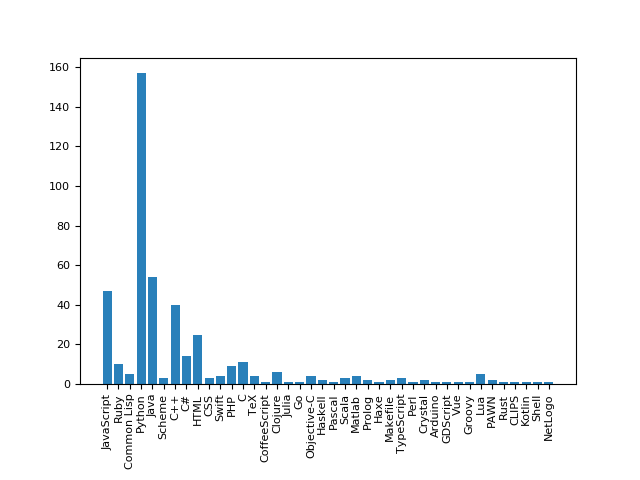
\includegraphics[width=1.0\textwidth]{img/ai-lang.png}
				\end{center}
			\end{figure}
		\end{column}
		\begin{column}{0.5\paperwidth}
			\begin{figure}[h]
				\begin{center}
					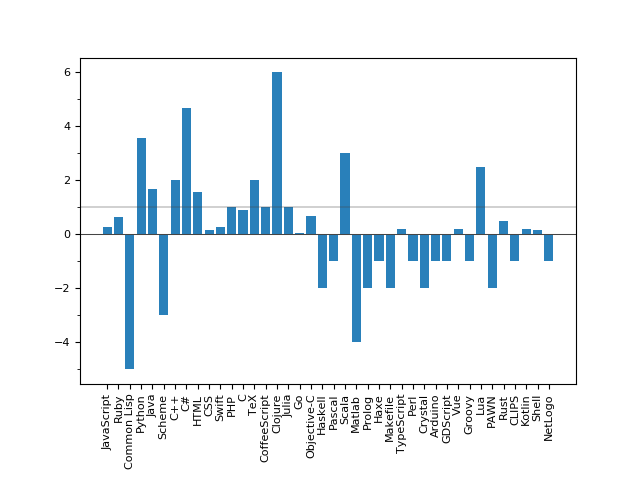
\includegraphics[width=1.0\textwidth]{img/proportion-lang.png}
				\end{center}
			\end{figure}
		\end{column}
	\end{columns}
	\bigskip
	\bigskip
	\centering
	¿Las diferencias son debidas al lenguaje o a las herramientas?
	\bigskip
	\bigskip
\end{frame}

\begin{frame}{Elementos de un lenguaje especializado en IA}
	\begin{itemize}
		\item Compilación AOT \\
		\bigskip
		\item Recolección de basura \\
		\bigskip
		\item Tipos graduales \\
		\bigskip
		\item Concurrencia mediante paso de mensajes \\
		\bigskip
		\item Facilidades a la computación simbólica \\
		\bigskip
		\item Facilidades al álgebra lineal \\
	\end{itemize}
\end{frame}

\section{Objetivos}
\begin{frame}{Objetivos}
	\begin{itemize}
		\item Introducir la teoría de lenguajes de programación\\
		\bigskip
		\item Relacionar la teoría de tipos y los sistemas de tipos\\
		\bigskip
		\item Diseñar un lenguaje especializado en inteligencia artificial\\
		\bigskip
		\item Implementar el compilador de dicho lenguaje\\
	\end{itemize}
\end{frame}

\section{Fundamentos matemáticos}

\begin{frame}{Teoría de lenguajes de programación}
	Rama de las ciencias de la computación que estudia distintos aspectos de los lenguajes de programación\\
	\bigskip
	
	\begin{itemize}

		\item Cómo diseñar lenguajes\\
		\bigskip
		\item Cómo formalizar lenguajes\\
		\bigskip
		\item Cómo implementar lenguajes\\
		\bigskip
		\item Se apoya en teorías matemáticas como el calculo lambda, la teoría de tipos o la teoría de categorías\\
	\end{itemize}
	\bigskip
\end{frame}


\begin{frame}{Teoría de tipos}
	Formalismo matemático que puede servir como fundamentación de las matemáticas\\
	\bigskip
	\begin{itemize}
		\item Todo es un tipo, menos los términos
		\[a\ \colon A\ \ 
		\begin{cases} 
		a \text{ es evidencia de } A
\\
		a \in A
		\end{cases}
		\]
		
		\item No existe el conjunto de todos los conjuntos. Se utiliza una torre de universos $U_1 : U_2 : ... : U_i : ...$\\
		
		$$\text{Ya no tiene sentido plantear } A = \{X \mid X \notin X\}$$
		
	\end{itemize}
	\bigskip
\end{frame}


\begin{frame}
	\begin{itemize}
		\item $\text{Tipo } A \to B$\\
		
		$$\text{Se construye como } \lambda(x:A).\Phi\ :A \to B \text{ si } \Phi:B \text{ cuando } x:A$$
		$$\text{Se le da el nombre } f:A \to B \text{ con } f :\equiv \lambda(x:A).\Phi$$
		$$\text{Se utiliza con } f(a) \text{ si } a:A$$
		\smallskip
		
		\item Tipo $A \times B$\\
		
		$$\text{Se construye como } (a, b):A \times B \text{ si } a:A \text{ y } b:B$$
		$$\text{Se utiliza con } f((a, b)) :\equiv (g(a))(b) \text{ dado un } g:A \to B \to C$$
	\end{itemize}
\end{frame}

\begin{frame}
	\begin{itemize}
		\item Tipo $\Pi_{(x:A)} B(x)$\\
		$$\text{Dados } A:U \text{ y } B:A \to U \text{ se construye } f:\Pi_{(x:A)} B(x)$$
		$$\text{ con } f:\equiv\lambda(x:A).\Phi \text{ con la diferencia de que } f(a):B(a)$$
		\smallskip
		
		\item Tipo $\Sigma_{(x:A)} B(x)$\\
		$$\text{Dados } a:A \text{ y } b:B(a) \text{ se construye como } (a, b):\Sigma_{(x:A)} B(x)$$
	\end{itemize}
	
\end{frame}


\begin{frame}{Cálculo lambda}
	\vspace{-0.5cm}
	$$(\lambda x.xx)\lambda x.xz$$
	\smallskip
	
	\begin{columns}
		\hspace{-2.2cm}
		\begin{column}{0.5\paperwidth}
			\begin{grammar}{t}{términos}
				x\\
				\lambda x.t\\
				t\ t
			\end{grammar}
			\smallskip
			\begin{grammar}{v}{valores}
				\lambda x.t
			\end{grammar}
		\end{column}
	
		\hspace*{-0.5cm}
		\begin{column}{0.5\paperwidth}
			\[\inference[]{t_1 -> t_1'}{t_1\ t_2 -> t_1'\ t_2}\]
			\smallskip
			\[\inference[]{t_2 -> t_2'}{v_1\ t_2 -> v_1\ t_2'}\]
			\smallskip
			\[\inference[]{}{(\lambda x.t_{12})v_2 -> [x \mapsto v_2]t_{12}}\]
		\end{column}
	\end{columns}
	\smallskip
	\smallskip
	\bigskip
	$$(\lambda x.xx)(\lambda x.xz) -> (\lambda x.xz)(\lambda x.xz) -> (\lambda x.xz)z$$
	\bigskip
	
\end{frame}

\begin{frame}{Cálculo lambda simplemente tipado}
	\vspace*{-0.5cm}
	$$true : Bool$$
	$$(\lambda x :
Bool.x)true$$
	\smallskip
	
	\begin{columns}
		\hspace{1cm}
		\begin{column}{0.5\paperwidth}
			\begin{grammar}{t}{términos}
				x\\
				\lambda x\textcolor{myred}{:T}.t\\
				t\ t
			\end{grammar}
			\begin{grammar}{v}{valores}
				\lambda x\textcolor{myred}{:T}.t
			\end{grammar}
			{\color{myred}
				\begin{grammar}{\textcolor{myred}{T}}{\textcolor{myred}{tipos}}
					T \to T &
				\end{grammar}
			}
			{\color{myred}
				\begin{grammar}{\Gamma}{contexto}
					\o    &  \\
					\Gamma,x:T
			\end{grammar}}
		\end{column}
		
		\hspace*{-2.2cm}
		\begin{column}{0.5\paperwidth}
			\[\inference[T-Var:]{x:T \in \Gamma}{\Gamma |- x:T}\]
			
			\[\inference[T-Abs:]
			{\Gamma,x:T_1 |- t_2:T_2}
			{\Gamma |- \lambda x:T_1.t2\ :\ T_1 -> T_2}
			\]
			
			\[\inference[T-Ap:]
			{\Gamma |- t_1:T_{11}->T_{12}\ \ \Gamma |- t_2:T_{11}}
			{\Gamma |- t_1\ t_2:T_{12}}
			\]
		\end{column}
	\end{columns}
\end{frame}

\begin{frame}{Seguridad = Progreso + Preservación}
	\begin{block}{Seguridad}
		Un sistema de tipos es seguro (y por extensión el lenguaje que lo contiene) si cualquier término bien tipado nunca se queda atascado
	\end{block}

	\bigskip

	\begin{block}{Progreso}
		Si un término está bien tipado no se encuentra atascado
	\end{block}

	\bigskip

	\begin{block}{Preservación}
		Si un término está bien tipado, tras un paso de cálculo lo sigue estando
	\end{block}
\end{frame}

\begin{frame}{Funciones $\mu$-recursivas y turing-completitud}
	\begin{itemize}
		\item Funciones constantes
		\begin{equation*}
		\begin{aligned}[c]
		&f \colon \mathbb{N}^k \to \mathbb{N}\\
		&f(x_1,...,x_k) \mapsto n \\
		\end{aligned}
		\end{equation*}
		
		\item Función sucesor
		\begin{equation*}
		\begin{aligned}[c]
		&S \colon \mathbb{N} \to \mathbb{N}\\
		&S(x) \mapsto x + 1 \\
		\end{aligned}
		\end{equation*}
		
		\item Funciones proyección
		\begin{equation*}
		\begin{aligned}[c]
		&P_i^k \colon \mathbb{N}^k \to \mathbb{N}\\
		&P_i^k(x_1, ..., x_k) \mapsto x_i \\
		\end{aligned}
		\end{equation*}
		
	\end{itemize}
\end{frame}
\begin{frame}	
	\begin{itemize}
		\item El operador de composición ($\circ$), sobre una función $h(x_1, ..., x_m)$ y $m$ funciones $g_i(x_1, ..., x_k)$
		$$(h \circ (g_1, ..., g_m))(x_1, ..., x_k) = h(g_1(x_1, ..., x_k), ..., g_m(x_1, ..., x_k))$$
		
		\bigskip
		\item El operador de recursión primitiva ($\rho$), sobre dos funciones $g(x_1, ..., x_k)$ y $h(y,z,x_1, ..., x_k)$
		\begin{align*}
		&\rho(g, h)(0, x_1, ..., x_k) = g(x_1, ..., x_k)\\
		&\rho(g, h)(y+1, x_1, ..., x_k) = h(y, \rho(g, h)(y, x_1, ..., x_k), x_1, ..., x_k)
		\end{align*}
		
		\bigskip
		\item El operador de minimización ($\mu$), sobre una función $f(y, x_1, ..., x_k)$
		\[
		\mu(f)(x_1, ..., x_k) = z \Leftrightarrow
		\begin{cases}
		f(z, x_1, ..., x_k) = 0\\
		f(i, x_1, ..., x_k) > 0 &\forall\ 0 \leq i \leq z-1
		\end{cases}
		\]
		
	\end{itemize}
\end{frame}

\section{Propuesta de lenguaje: \textit{tail}}


\begin{frame}{Propuesta de lenguaje: \textit{tail}}
	{\centering The Artificial Intelligence Language}
	\begin{columns}
		\begin{column}{0.35\paperwidth}
			\begin{figure}[h]
				\begin{center}
					
\includegraphics[width=0.7\textwidth]{img/logo.png}
				\end{center}
			\end{figure}
		\end{column}
		\begin{column}{0.65\paperwidth}
			\begin{itemize}
				\item Unión e intersección de tipos graduales\\
				\smallskip
				\smallskip
				\item Captura de variables no inicializadas \\
				\smallskip
				\smallskip
				\item Átomos\\
				\smallskip
				\smallskip
				\item Variants generalizadas\\
				\smallskip
				\smallskip
				\item Tuplas como argumento\\
				\smallskip
				\smallskip
				\item Sobrecarga de funciones y operadores\\
				\smallskip
				\smallskip
				\item Números complejos y racionales\\
			\end{itemize}
		\end{column}
	\end{columns}
\end{frame}

\begin{frame}[fragile]{Algunas características destacables}
	\begin{lstlisting}[style=tail]
	f : Bool, ? -> ? or Int
	f(b, x) := if b then x else 1
	
	f(True, "hola")
	\end{lstlisting}
	
	\begin{lstlisting}[style=tail]
	f : :Complejo or :Racional -> Complex or Rational
	f(a) := if a = :complejo then 2 + 3i else 3//4
	
	f(:compeljo) # Error en tiempo de compilación
	
	x : Atom := :cualquier_atomo
	\end{lstlisting}

\end{frame}

\begin{frame}[fragile]{Algunas características destacables}
	\vspace{0.4cm}
	\begin{lstlisting}[style=tail]
	variant Point :: Point(x, y) : Real, Real
	               
	@+@ (p1, p2) := Point::Point(p1.x + p2.x, p1.y + p2.y)
	\end{lstlisting}
	\vspace{-0.4cm}
	\begin{lstlisting}[style=tail]
	x := [1 2 3 | 4 5 6 || 7 8 9]
	
	x := [ 1 2 3 |
	     | 4 5 6 |
	     | 7 8 9 ]
	\end{lstlisting}
	\vspace{-0.4cm}
	\begin{lstlisting}[style=tail]
	f(x) := x, x+1, x+2
	g(a, b, c) := a + b + c
	
	g(f(1))
	\end{lstlisting}	
\end{frame}

\begin{frame}{Algunas características destacables}
	{Unión e intersección de tipos graduales}
	Con tipado estático la relación de subtipado $\leq$ es la inclusión
	
	\[\gamma \colon GTypes \to \mathcal{P}(STypes)\]
	
	\vspace{-0.6cm}
	\begin{columns}
		\begin{column}{0.5\paperwidth}	
			\begin{align*}
			\gamma(?) &\mapsto STypes \\
			\gamma(B) &\mapsto \{B\} \\
			\gamma(Void) &\mapsto \{Void\} \\
			\gamma(U) &\mapsto \{U\} \\
			\end{align*}
		\end{column}
		\hspace{-2cm}
		\begin{column}{0.5\paperwidth}
			\begin{align*}
			\gamma(\tau_1 -> \tau_2) &\mapsto \{T_1 -> T_2 \mid T_i \in \gamma(\tau_i)\} \\	
			\gamma(\tau_1 \text{ or } \tau_2) &\mapsto \{T_1 \text{ or } T_2 \mid T_i \in \gamma(\tau_i)\} \\
			\gamma(\tau_1 \text{ and } \tau_2) &\mapsto \{T_1 \text{ and } T_2 \mid T_i \in \gamma(\tau_i)\} \\
			\gamma(\text{not } T) &\mapsto \{\text{not } T\} \\
			\end{align*}
		\end{column}
	\end{columns}

	\begin{block}{Gradual Extrema}
		Para todo tipo gradual $\tau \in GTypes$ existen dos tipos estáticos $\tau^{\Uparrow}$ y $\tau^{\Downarrow}$ tal que para todo $T \in \gamma(\tau),\ \tau^{\Downarrow} \leq T \leq \tau^{\Uparrow}$
	\end{block}
\end{frame}

\begin{frame}{Algunas características destacables}
	{Unión e intersección de tipos graduales}
	\vspace{-0.5cm}
	\begin{block}{Extensión de la relación de subtipado}
		Para cada par $\sigma$, $\tau$ de tipos graduales definimos la relación $\widetilde{\leq}$ como:
		$$\sigma \widetilde{\leq} \tau \Leftrightarrow \sigma^{\Downarrow} \leq \tau^{\Uparrow}$$\\
		
		Para cada par $\sigma$, $\tau$ de tipos graduales definimos la relación $\widetilde{\nleq}$ como:
		$$\sigma \widetilde{\nleq} \tau \Leftrightarrow \sigma^{\Uparrow} \nleq \tau^{\Downarrow}$$\\
	\end{block}
\end{frame}

\begin{frame}{Algunas características destacables}
	{Propiedades del lenguaje}
	\begin{block}{}
		Se puede demostrar que tail es turing-completo usando funciones $\mu$-recursivas
	\end{block}
	\bigskip
	\bigskip
	\begin{block}{}
		Se puede demostrar que tail es un lenguaje seguro si todos sus términos están tipados de forma estática
	\end{block}
\end{frame}

\begin{frame}[fragile]{Ejemplos de ejecución}
	\begin{columns}
		\begin{column}{0.47\paperwidth}
			\begin{lstlisting}[style=tail]
x : Int
			
			
write("fib(x) = {fib(x)}")
			\end{lstlisting}
			
			\begin{figure}[h]
				\begin{center}
					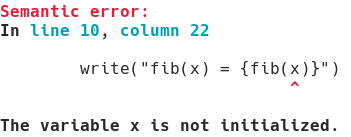
\includegraphics[width=0.9\textwidth]{img/fib4.png}
				\end{center}
			\end{figure}
		\end{column}
	
		\begin{column}{0.47\paperwidth}
			\vspace{0.23cm}
			\begin{lstlisting}[style=tail]
x : (:A1 or :A2 ) and
    (:A2 or :A3 )
			
x := :a3
			\end{lstlisting}
			
			\begin{figure}[h]
				\begin{center}
					\hspace*{-0.8cm}
					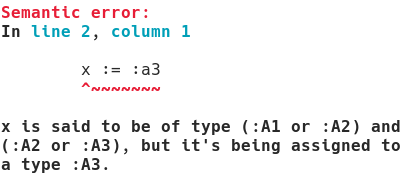
\includegraphics[width=0.9\textwidth]{img/int2.png}
				\end{center}
			\end{figure}
		\end{column}
	\end{columns}
\end{frame}

\section{Conclusiones y trabajo futuro}

\begin{frame}{Conclusiones y trabajo futuro}
	{Conclusiones}
	\begin{itemize}
		\item Hemos presentado la teoría de lenguajes de programación
		\bigskip
		\item Hemos estudiado la aplicación práctica de la teoría de tipos
		\bigskip
		\item Hemos diseñado un lenguaje especializado en inteligencia artificial
		\bigskip
		\item Hemos aplicado los resultados teóricos estudiados al análisis de nuestro lenguaje
		\bigskip
		\item Hemos implementado parcialmente su compilador
	\end{itemize}
\end{frame}

\begin{frame}{Conclusiones y trabajo futuro}
	{Trabajo futuro}
	\begin{itemize}
		\item Completar la fase de generación de código
		\bigskip
		\item Diseñar un sistema de módulos para tail
		\bigskip
		\item Implementar un modelo de programación concurrente
		\bigskip
		\item Estudiar en profundidad los tipos dependientes
	\end{itemize}
\end{frame}

\begin{frame}
	\Huge \centering ¿Alguna pregunta?
\end{frame}

\end{document}
